\section{HITS Algorithm} \label{sec:HITS}
The Hypertext Induced Topic Search (HITS) algorithm was developed by Jon Kleinburg, and is similar to PR as it ranks web pages by popularity, however HITS produces two popularity scores, for each web page.  Kleinburg developed this algorithm as a connectivity analysis on the hyper linked environment of the web. The algorithm manages to distil a broad topic down to a representation of a very small size \cite{kleinberg1999authoritative}. 

The HITS algorithm defines an authoritative page as a page with sources of information on a topic, while a hub is a page that is not in itself a source of information, but compilations to authoritative pages \cite{manning}. Authoritative pages have many inlinks, whilst a hub has many outlinks, each web page on a graph has some measure of an authority and some measure of a hub. A good authority is one which is pointed to by good hubs, whilst a good hub is one which points to good authorities. This cyclic definition is similar to the definition for PR, and we use an iterative computation in order to rank the web pages in the same manner.

The authority weight of a page is the sum of the hubness weights of its parents, which are the backlinks of a node, whilst the hubness weight of a page is the sum of the authority weights of its children, the forward links from a node \cite{baldi2003modeling}.

{Authorities are pages with good coverage of a topic, hubs are pages with links to many useful pages on a topic \cite{bonato}.} 

HITS was developed as a way to combat two problems that can occur when ranking web pages. One of these is the scarcity problem, where not many pages contain the exact information that you desire, and it can be difficult to identify the web pages that the user requires. The second problem that can occur is the abundance problem, where the number of pages that are returned to the user as being relevant to the query is too much for the human user to digest. 



\subsection{HITS Implementation} \label{sec:HITS implementation}
The HITS algorithm consists of two steps, the first step involves building a neighbourhood graph, N, which is related to the query term, and is known as the sampling step. The second step, the weight-propagation step, involves the computation of the authority and hub scores for each page, two ranked lists are then presented to the user. This computation is an iterative calculation, where firstly each page is assigned an initial authority score $x_i^{(0)}$ and an initial hub score $y_i^{(0)}$, which are redefined by computing \begin{equation} \label{eq:HITS1}
x_i^{(k)} = \displaystyle \sum_{j:e_{ij}\in E} y_j^{(k-1)} \quad\mathrm{and}\quad y_i^{(k)} = \displaystyle \sum_{j:e_{ij}\in E} x_j^{(k)}  \quad\mathrm{for}\quad k=1,2,3\ldots
\end{equation} 

In the sampling step, the algorithm first creates a root set of pages which contain the query, \textit{q}. Next a base set of pages is formed which includes the root set along with any pages which point into the root set, or which are pointed to, as displayed by Figure \ref{fig:HITS expanding}. 
\begin{figure}[h]
\centering
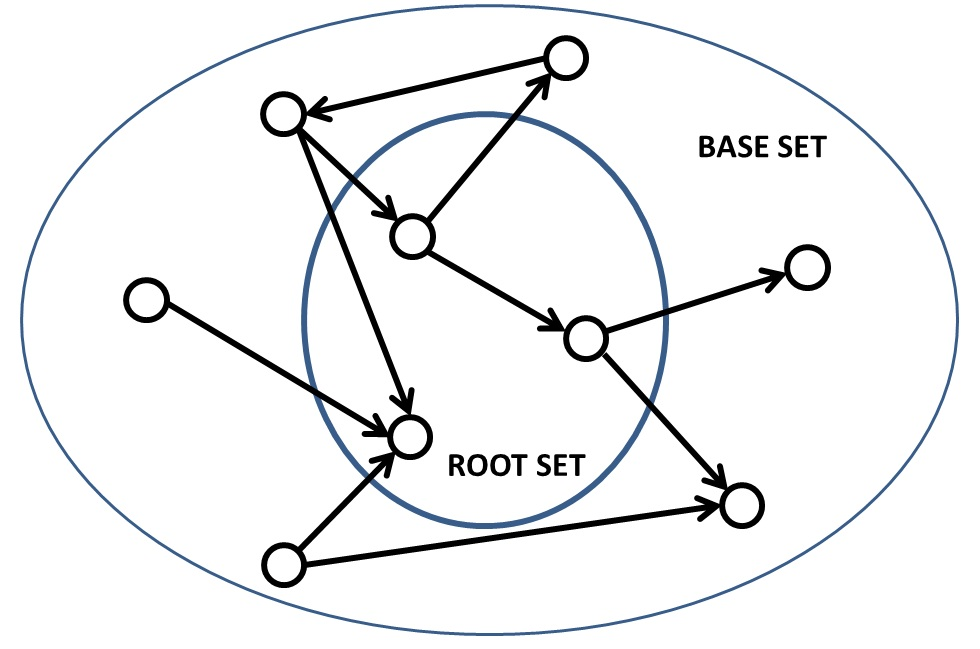
\includegraphics[width=5cm]{expanding_root.jpg}
\caption{Expanding the root set into the base set, taken from \cite{pict}}
\label{fig:HITS expanding}
\end{figure}
This expansion usually resolves the issue of synonyms, along with the issue that good authoritative pages may not contain the query item. The base set can become very large and so in practice a maximum number of inlinking and outlinking pages that are added for a particular node in the root set is fixed, for example at 100. 

The base set is constructed in this manner for several reasons, firstly a good authority page may not contain the query term  as there may be synonyms more commonly used. Also, if the root set contains a good hub set, this expansion means that the base set will then containing good authority pages that it may not have captured previously. The base set then forms the neighbourhood graph, N, which is then used in the computation of the authority and hub scores for all pages in N.


The first step in the weight-propagation step is the formation of the adjacency matrix \textbf{L}, where \[\textbf{L}_{ij} = \begin{cases} 1, & \textnormal{if there exists an edge from node \textit{i} to node \textit{j}}\\ 0 & \textnormal{otherwise}
\end{cases}\]
If we use the example in Figure \ref{fig:Example} as N for the following calculations, we are able to generate the following adjacency matrix:
\begin{equation*}
\textbf{L}=\left(
\begin{array}{cccccccc}
0 & 1 & 0 & 1 & 0 & 1 & 0 & 0 \\
0 & 0 & 1 & 0 & 1 & 0 & 0 & 0 \\
0 & 0 & 0 & 0 & 1 & 0 & 0 & 0 \\
0 & 0 & 0 & 0 & 1 & 0 & 1 & 0 \\
0 & 0 & 0 & 0 & 0 & 0 & 0 & 1 \\
0 & 0 & 0 & 1 & 0 & 0 & 1 & 1 \\
0 & 0 & 0 & 0 & 0 & 0 & 0 & 0 \\
0 & 0 & 0 & 0 & 1 & 0 & 1 & 0 \\
\end{array}
\right)
\end{equation*} 

We are able to represent Equations \eqref{eq:HITS1} in terms of this adjacency matrix as \begin{equation} \label{eq:HITSMatrix}
\textbf{x}^{(k)} = \textbf{L}^T\textbf{y}^{(k-1)}\quad\mathrm{and}\quad \textbf{y}^{(k)}=\textbf{Lx}^{(k)}
\end{equation} where \(\textbf{x}^{(k)}\) and \(\textbf{y}^{(k)}\) are $[\textit{n}\times 1]$ vectors which hold the approximate authority and hub scores at each iteration respectively. In the HITS algorithm, we first initialise $\textbf{y}^{(0)}$ = \textbf{e}, where \textbf{e} is the column vector of all ones, and then apply Equations \eqref{eq:HITSMatrix} until convergence. 

We are able to further simplify Equations \eqref{eq:HITSMatrix} to \begin{equation} \label{eq:HITSSimplify}
\textbf{x}^{(k)} = \textbf{L}^T\textbf{Lx}^{(k-1)}\quad\mathrm{and}\quad \textbf{y}^{(k)}=\textbf{LL}^T\textbf{y}^{(k-1)}
\end{equation} and this shows that we able to use the iterative power method on the matrices $\textbf{L}^T\textbf{L}$ and $\textbf{LL}^T$ respectively. The HITS algorithm defines the matrix $\textbf{L}^T\textbf{L}$ as the Authority matrix, and $\textbf{LL}^T$ as the Hub matrix. So when we apply the power method to these matrices, we compute the authority vector \textbf{x}, which contains the authority scores for all pages in the base set, and the hub vector, \textbf{y}, which similarly contains the hub scores.

Continuing to use Figure \ref{fig:Example} as our example, we are able to produce the following matrices;
\begin{equation*}
%\textnormal{Authority matrix} =
\textbf{L}^T\textbf{L}=\left(
\begin{array}{cccccccc}
0 & 0 & 0 & 0 & 0 & 0 & 0 & 0 \\
0 & 1 & 0 & 1 & 0 & 1 & 0 & 0 \\
0 & 0 & 1 & 0 & 1 & 0 & 0 & 0 \\
0 & 1 & 0 & 2 & 0 & 1 & 1 & 1 \\
0 & 0 & 1 & 0 & 4 & 0 & 2 & 0 \\
0 & 1 & 0 & 1 & 0 & 1 & 0 & 0 \\
0 & 0 & 0 & 1 & 2 & 0 & 3 & 1 \\
0 & 0 & 0 & 1 & 0 & 0 & 1 & 2 \\
\end{array}
\right)
\mathrm{,}\quad\mathrm{and}\quad
%\textnormal{Hub matrix} =
\textbf{LL}^T=\left(
\begin{array}{cccccccc}
3 & 0 & 0 & 0 & 0 & 1 & 0 & 0 \\
0 & 2 & 1 & 1 & 0 & 0 & 0 & 1 \\
0 & 1 & 1 & 1 & 0 & 0 & 0 & 1 \\
0 & 1 & 1 & 2 & 0 & 1 & 0 & 2 \\
0 & 0 & 0 & 0 & 1 & 1 & 0 & 0 \\
1 & 0 & 0 & 1 & 1 & 3 & 0 & 1 \\
0 & 0 & 0 & 0 & 0 & 0 & 0 & 0 \\
0 & 1 & 1 & 2 & 0 & 1 & 0 & 2 \\
\end{array}
\right)
\end{equation*} Where we note that these matrices are symmetric, positive semi-definite and non-negative, and so HITS with normalization will always converge, with as few as 5 iterations required in order to compute fairly accurate ranking lists \cite{manning}. 

Using the power method, as the Matlab code given in Appendix \ref{app:code}, we are able to compute authority score \textbf{x}, and hub score, \textbf{y}, vectors
\begin{eqnarray}
\textbf{x}^T = \left( \begin{array} {cccccccc}
0 & 0.030 & 0.069 & 0.118 & 0.343 &0.030 &0.305 &0.106
\end{array}\right) \\
\textbf{y}^T = \left( \begin{array} {cccccccc}
0.062 & 0.144 & 0.120 & 0.226 & 0.037 & 0.185 & 0 & 0.226
\end{array}\right)
\end{eqnarray} Hence we are able to produce two ranked lists for the user in terms of the authority and hub values of the pages in N, as shown in Table \ref{Table:HITS}.

\begin{table}[h] \caption{HITS Authority and Hub rankings}
 \centering
 \begin{tabular} {c| c c} 
 Node & Authority & Hub \\ [0.5ex] 
 \hline
 1&8&6\\
 2&6&4\\
 3&5&5\\
 4&3&1\\
 5&1&7\\
 6&6&3\\
 7&2&8\\
 8&4&1\\
 \end{tabular}
 \label{Table:HITS}
\end{table} 

We are able to note that node 5 is the most authoritative page, this follows from the fact that node 5 has many inlinks. Node 5 is also given a low hub score, as it points only into node 8, which has average authority in the graph. Subsequently, node 8 has a high hub score, as it points into the authoritative node 5.